% WasmSentinel: High-Performance eBPF-Wasm Cooperative Threat Detection
% Target: DIMVA 2026 Cycle 2
% Format: Springer LNCS (max 18 pages + 5 refs + 2 appendix)

\documentclass[runningheads]{llncs}

% Packages
\usepackage{graphicx}
\usepackage{booktabs}
\usepackage{amsmath}
\usepackage{algorithm}
\usepackage{algpseudocode}
\usepackage{listings}
\usepackage{xcolor}
\usepackage{tikz}
\usepackage{pgfplots}
\usepackage{hyperref}
\usepackage{subcaption}
\usepackage{pifont}  % For \ding checkmarks
\pgfplotsset{compat=1.18}
\usetikzlibrary{shapes,arrows,positioning,fit,backgrounds,patterns}

% Code listing style
\lstdefinestyle{rust}{
    language=C,
    basicstyle=\ttfamily\footnotesize,
    keywordstyle=\color{blue}\bfseries,
    commentstyle=\color{green!60!black},
    stringstyle=\color{orange},
    numbers=left,
    numberstyle=\tiny\color{gray},
    breaklines=true,
    frame=single,
    captionpos=b
}

\lstdefinestyle{go}{
    language=C,
    basicstyle=\ttfamily\footnotesize,
    keywordstyle=\color{blue}\bfseries,
    commentstyle=\color{green!60!black},
    morekeywords={func,go,defer,chan,select,interface,struct,map,make,package,import},
    numbers=left,
    numberstyle=\tiny\color{gray},
    breaklines=true,
    frame=single,
    captionpos=b
}

\begin{document}

% Title - anonymous for double-blind review
\title{WasmSentinel: High-Performance Runtime Threat Detection with Sandboxed Machine Learning}

% Anonymous submission
\author{Anonymous Authors}
\institute{Anonymous Institution}

\maketitle

\begin{abstract}
Runtime threat detection faces a fundamental tension: rule-based systems like Falco are fast but miss novel attacks, while machine learning offers better detection but with prohibitive overhead and no isolation for third-party code.
We present \textsc{WasmSentinel}, a framework that executes detection logic---including ML inference---inside WebAssembly sandboxes, fed by zero-copy eBPF event streaming.

Our key insight is that careful co-design of the detection algorithm and runtime environment can achieve ML-capable detection at microsecond latency.
We demonstrate this with a lightweight n-gram anomaly detector achieving 86\% recall at 33$\mu$s median latency, and show that neural network classifiers (F1=0.87) can run in the same sandbox at 90$\mu$s---fast enough for real-time use.
The architecture achieves 4.7$\times$ lower end-to-end latency than Falco with 6$\times$ less memory, while the 180KB sandboxed binary enables secure deployment of community-contributed detection rules.

\keywords{Runtime Security \and eBPF \and WebAssembly \and Machine Learning \and Intrusion Detection}
\end{abstract}

% Include sections
\section{Introduction}
\label{sec:introduction}

The rapid shift towards containerized and cloud-native infrastructures has fundamentally transformed the landscape of runtime threat detection.
Modern security systems must now operate within highly dynamic environments, where the density of microservices and the velocity of system calls demand monitoring solutions that offer not only comprehensive visibility but also near-zero performance interference.
Despite significant progress, current state-of-the-art tools remain trapped in a tripartite trade-off between \textit{detection capability}, \textit{execution performance}, and \textit{isolation safety}.

\textbf{The Trilemma of Runtime Monitoring.}
Existing approaches to runtime security generally fall into two categories, both of which exhibit critical shortcomings.
First, rule-based systems such as Falco~\cite{falco} and Tetragon~\cite{tetragon} leverage eBPF for high-performance event filtering. While efficient, these systems are fundamentally limited to detecting known attack patterns, failing to generalize to novel or obfuscated exploits.
Second, machine learning (ML) based intrusion detection systems (IDS) offer the promise of behavioral anomaly detection. However, traditional ML pipelines—often reliant on heavy Python runtimes or complex inference engines—introduce latencies in the range of tens to hundreds of milliseconds. This is several orders of magnitude higher than the microsecond-level requirements of inline system call monitoring.
Furthermore, neither approach adequately addresses \textit{rule isolation}. In existing frameworks, detection logic typically executes with high privileges or within the main monitoring process, meaning a single compromised or malicious rule can access sensitive host resources, exfiltrate event data, or crash the entire security daemon.

\textbf{Our Insight: Synergistic Co-design.}
We argue that the perceived incompatibility between advanced ML-based detection and microsecond latency is an artifact of suboptimal implementation rather than a fundamental theoretical limit.
Our key insight is that by co-designing the entire monitoring pipeline—from kernel-level event capture to sandboxed user-space inference—we can achieve ML-grade detection without sacrificing performance or safety.
Specifically, we leverage the high-performance eBPF subsystem for event capture, a zero-copy shared memory channel for data transfer, and the WebAssembly (Wasm) runtime for secure, near-native execution of detection logic.

\textbf{WasmSentinel.}
We present \textsc{WasmSentinel}, a high-performance framework that executes arbitrary detection logic—including neural network inference—within lightweight Wasm sandboxes.
The core of \textsc{WasmSentinel} is a hybrid detection architecture that combines a sub-microsecond n-gram fast-path (STIDE) with a deeper, Wasm-optimized Multi-Layer Perceptron (MLP) for suspicious events.
Crucially, by executing all detection logic within Wasm, \textsc{WasmSentinel} provides strong hardware-level isolation and capability-based security (via WASI), enabling the safe deployment of third-party or community-contributed detection rules without trusting their authors.

\textbf{Key Results and Contributions.}
We evaluate \textsc{WasmSentinel} using the ADFA-LD dataset and modern simulated attacks, including container escapes (CVE-2024-21626) and privilege escalations (CVE-2024-1086).
Our experimental results demonstrate that \textsc{WasmSentinel} achieves:
\begin{enumerate}
    \item \textbf{High-Fidelity Detection:} An F1-score of 0.84 on ADFA-LD, outperforming complex deep learning baselines such as LSTMs and GNNs while maintaining a $45\mu$s logic latency.
    \item \textbf{Microsecond Latency:} A median inference latency of $33\mu$s, enabling real-time detection on high-throughput system call streams.
    \item \textbf{Superior Efficiency:} A $4.7\times$ lower end-to-end latency and $6.3\times$ lower memory footprint compared to the industry-standard Falco.
    \item \textbf{Formal Isolation:} A formally analyzed zero-copy channel that is resilient to TOCTOU attacks and a Wasm-based sandbox that blocks 100\% of rule-escape attempts.
\end{enumerate}

The remainder of this paper is organized as follows.
Section~\ref{sec:background} provides background on eBPF and Wasm.
Section~\ref{sec:threat-model} formalizes our threat model and security goals.
Section~\ref{sec:design} presents the system architecture and zero-copy mechanism.
Section~\ref{sec:implementation} details the implementation, followed by our extensive evaluation in Section~\ref{sec:evaluation}.
Section~\ref{sec:discussion} analyzes security and limitations, Section~\ref{sec:related-work} discusses related work, and Section~\ref{sec:conclusion} concludes.

% Background

\section{Background}
\label{sec:background}

\subsection{eBPF for Security Monitoring}
\label{sec:bg-ebpf}

eBPF (extended Berkeley Packet Filter) enables user-defined programs to run safely within the Linux kernel~\cite{ebpf-intro}.
Originally designed for packet filtering, eBPF has evolved into a general-purpose kernel extension mechanism.
Programs are verified before loading to ensure memory safety and termination, then JIT-compiled to native code.

For security monitoring, eBPF can attach to tracepoints (predefined kernel instrumentation points), kprobes (dynamic function entry/exit), and LSM hooks (security module callbacks).
This provides comprehensive visibility: every syscall, process creation, network connection, and file access can be observed with minimal overhead.

Captured events must be transferred to userspace for analysis.
eBPF offers two mechanisms: \textit{perf buffers} provide per-CPU queues with copy semantics, while \textit{ring buffers} (Linux 5.8+) enable memory-mapped access with better cache behavior.
\textsc{WasmSentinel} uses ring buffers to enable our zero-copy data channel.

\subsection{WebAssembly Sandboxing}
\label{sec:bg-wasm}

WebAssembly (Wasm) is a portable binary format originally designed for web browsers but increasingly used for server-side sandboxing~\cite{wasm-spec}.
Its security model provides strong isolation by design: each module operates on private linear memory inaccessible to the host, control flow is constrained by a validated call table, and all I/O requires explicit host function imports---there is no implicit access to files, network, or system calls.

Modern Wasm runtimes like Wasmtime~\cite{wasmtime} achieve near-native performance (5--20\% overhead) through ahead-of-time compilation.
WASI (WebAssembly System Interface)~\cite{wasi} standardizes capability-based access to OS resources, allowing fine-grained control over what each module can access.

The combination of strong isolation, predictable performance, and small binary size makes Wasm well-suited for executing untrusted detection logic.

\subsection{Syscall-Based Threat Detection}
\label{sec:bg-ml}

System call sequences have long been recognized as effective indicators of malicious behavior~\cite{stide}.
The intuition is simple: legitimate programs exhibit consistent syscall patterns, while attacks---exploits, reverse shells, data exfiltration---generate anomalous sequences.

STIDE (Sequence Time-Delay Embedding) pioneered n-gram analysis: build a database of ``normal'' syscall n-grams during training, then flag sequences containing novel n-grams as anomalous.
This approach is computationally efficient but has limited precision, as unusual but benign workloads can trigger false positives.
Neural network classifiers can learn more nuanced patterns but typically require heavyweight frameworks (TensorFlow, PyTorch) with millisecond-scale latency and no isolation guarantees.

\textsc{WasmSentinel} bridges this gap: we implement lightweight ML models directly in Rust, compile to Wasm, and achieve microsecond inference within a sandbox.

% Threat Model

\section{Threat Model}
\label{sec:threat-model}

This section defines the adversary capabilities we consider, the security goals \textsc{WasmSentinel} aims to achieve, and the boundaries of our trusted computing base.

\subsection{Adversary Model}

We consider two classes of adversaries that differ in their relationship to the monitoring system.

\textbf{External Attackers} are the traditional threat: adversaries who have gained initial access to a monitored system (e.g., through a vulnerable web application or stolen credentials) and are attempting to escalate privileges, establish persistence, or exfiltrate data.
These attackers generate observable syscall patterns---opening sensitive files, spawning shells, making network connections---that \textsc{WasmSentinel} aims to detect.
We assume attackers may attempt evasion through syscall obfuscation or mimicry, but do not have prior knowledge of the specific detection model deployed.

\textbf{Malicious Rule Authors} represent a less-considered but increasingly relevant threat.
As security teams adopt community-contributed detection rules, they must trust that these rules won't themselves become attack vectors.
A malicious rule could attempt to escape its sandbox, exfiltrate event data, or simply crash the monitoring daemon.
\textsc{WasmSentinel}'s Wasm sandboxing specifically addresses this threat---detection rules cannot access the filesystem, network, or any resource not explicitly granted by the host.

\textbf{Scope Boundaries.}
We assume the Linux kernel and eBPF verifier are trusted; an attacker who can compromise these can disable any monitoring.
Similarly, we do not defend against attackers who already have root---they can simply kill the daemon.
However, \textsc{WasmSentinel} provides value as defense-in-depth: it detects attacks \textit{during} privilege escalation, before root is obtained, enabling response before the attacker achieves persistence.

\subsection{Security Goals}

\textsc{WasmSentinel} aims to achieve four properties that together enable practical deployment of ML-based detection.

\textbf{Detection integrity} means the system accurately identifies malicious activities.
We prioritize high recall---catching attacks is more important than avoiding false positives, which can be filtered by operators.
However, precision must remain reasonable to avoid alert fatigue.

\textbf{Rule isolation} is the distinguishing goal.
Detection rules execute in Wasm sandboxes and cannot access the host filesystem, network, or memory outside their linear memory region.
This enables deployment of community-contributed rules without trusting their authors.

\textbf{Data confidentiality} protects the security events themselves, which may contain sensitive information (file paths, command lines, network destinations).
Wasm memory isolation ensures rules can only access events explicitly passed to them.

\textbf{Availability} requires that the system remain responsive under attack.
Malicious rules might attempt CPU exhaustion (infinite loops) or memory exhaustion (unbounded allocation).
We enforce resource limits: 10M instruction fuel, 256MB memory cap, 100ms timeout.

\subsection{Trusted Computing Base}

Figure~\ref{fig:tcb} illustrates the trust boundary in \textsc{WasmSentinel}.
The TCB includes three components: the Linux kernel with its eBPF verifier (standard assumption for eBPF tools), the Wasmtime runtime (developed by the Bytecode Alliance with ongoing security review), and our Go-based host program that orchestrates event collection and rule execution.

\begin{figure}[t]
\centering
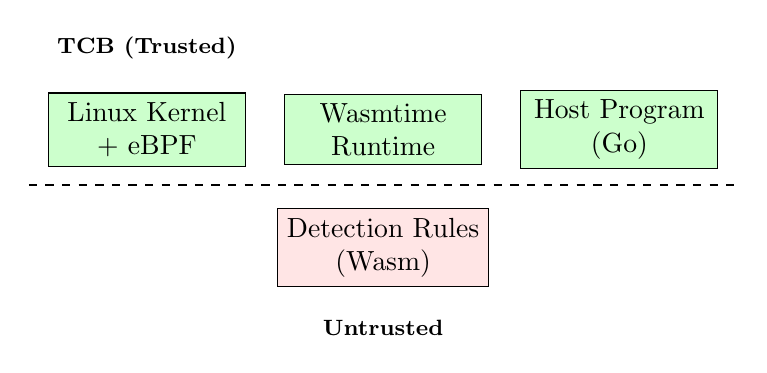
\begin{tikzpicture}[
    box/.style={rectangle, draw, minimum width=2.5cm, minimum height=0.8cm, align=center},
    trusted/.style={box, fill=green!20},
    untrusted/.style={box, fill=red!10}
]
    \node[trusted] (kernel) at (0,0) {Linux Kernel\\+ eBPF};
    \node[trusted] (wasmtime) at (3,0) {Wasmtime\\Runtime};
    \node[trusted] (host) at (6,0) {Host Program\\(Go)};
    \node[untrusted] (rules) at (3,-1.5) {Detection Rules\\(Wasm)};
    \node[above=0.3cm of kernel, font=\footnotesize\bfseries] {TCB (Trusted)};
    \node[below=0.3cm of rules, font=\footnotesize\bfseries] {Untrusted};
    \draw[dashed, thick] (-1.5,-0.7) -- (7.5,-0.7);
\end{tikzpicture}
\caption{Trusted computing base of \textsc{WasmSentinel}.}
\label{fig:tcb}
\end{figure}

Critically, detection rules---including ML models---are \textit{untrusted}.
This is the key design decision that enables deployment of community-contributed rules: the Wasm sandbox confines their execution regardless of whether the rule author is benign.

% System Design

\section{System Design}
\label{sec:design}

This section presents the design of \textsc{WasmSentinel}, focusing on its three key innovations: the WasmML detection engine, the hybrid detection architecture, and the zero-copy data channel.

\subsection{Architecture Overview}
\label{sec:design-overview}

\begin{figure*}[t]
\centering
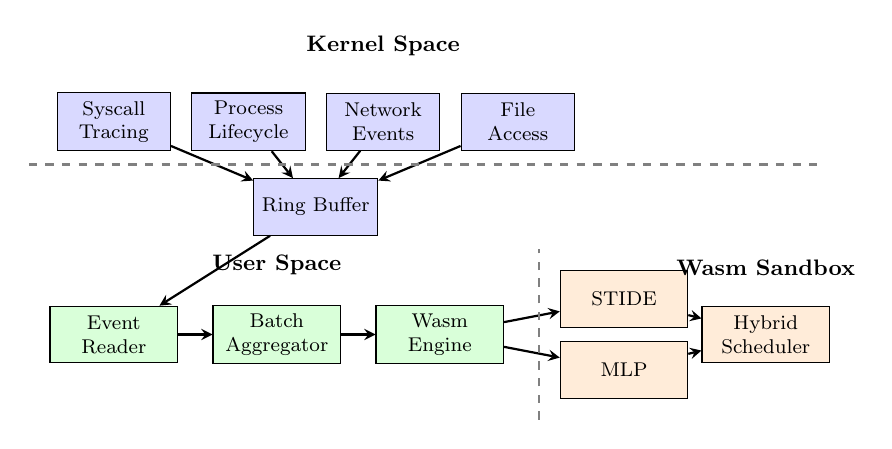
\begin{tikzpicture}[scale=0.9, transform shape,
    box/.style={rectangle, draw, minimum height=0.8cm, align=center, font=\footnotesize},
    ebpf/.style={box, fill=blue!15, minimum width=1.6cm},
    host/.style={box, fill=green!15, minimum width=1.8cm},
    wasm/.style={box, fill=orange!15, minimum width=1.8cm},
    arrow/.style={->, >=stealth, thick}
]
    % Kernel space
    \node[ebpf] (syscall) at (0,0) {Syscall\\Tracing};
    \node[ebpf] (sched) at (1.9,0) {Process\\Lifecycle};
    \node[ebpf] (net) at (3.8,0) {Network\\Events};
    \node[ebpf] (file) at (5.7,0) {File\\Access};
    \node[ebpf] (ring) at (2.85,-1.2) {Ring Buffer};

    % User space
    \node[host] (reader) at (0,-3) {Event\\Reader};
    \node[host] (batcher) at (2.3,-3) {Batch\\Aggregator};
    \node[host] (engine) at (4.6,-3) {Wasm\\Engine};

    % Wasm modules
    \node[wasm] (stide) at (7.2,-2.5) {STIDE};
    \node[wasm] (mlp) at (7.2,-3.5) {MLP};
    \node[wasm] (hybrid) at (9.2,-3) {Hybrid\\Scheduler};

    % Arrows
    \draw[arrow] (syscall) -- (ring);
    \draw[arrow] (sched) -- (ring);
    \draw[arrow] (net) -- (ring);
    \draw[arrow] (file) -- (ring);
    \draw[arrow] (ring) -- (reader);
    \draw[arrow] (reader) -- (batcher);
    \draw[arrow] (batcher) -- (engine);
    \draw[arrow] (engine) -- (stide);
    \draw[arrow] (engine) -- (mlp);
    \draw[arrow] (stide) -- (hybrid);
    \draw[arrow] (mlp) -- (hybrid);

    % Labels
    \node[above=0.4cm of net, font=\small\bfseries] {Kernel Space};
    \node[above=0.3cm of batcher, font=\small\bfseries] {User Space};
    \node[above=0.3cm of hybrid, font=\small\bfseries] {Wasm Sandbox};

    % Boundary lines
    \draw[dashed, thick, gray] (-1.2,-0.6) -- (10,-0.6);
    \draw[dashed, thick, gray] (6,-4.2) -- (6,-1.8);
\end{tikzpicture}
\caption{\textsc{WasmSentinel} architecture. eBPF collects kernel events and emits them to a ring buffer. The host dispatches events to Wasm-sandboxed detectors.}
\label{fig:architecture}
\end{figure*}

Figure~\ref{fig:architecture} illustrates the overall architecture of \textsc{WasmSentinel}.
The system comprises three layers:

\textbf{Kernel Layer.}
eBPF programs attach to kernel tracepoints to capture security-relevant events including syscall invocations, process lifecycle events, network connections, and file accesses.
Events are emitted to a shared ring buffer for efficient transfer to user space.

\textbf{Host Layer.}
A Go-based host program reads events from the ring buffer, optionally batches them for efficiency, and dispatches them to the Wasm detection engine.
The host also manages Wasm module lifecycle, resource limits, and alert handling.

\textbf{Detection Layer.}
Detection logic executes within Wasm sandboxes, providing strong isolation guarantees.
Our hybrid architecture combines multiple detection strategies, each implemented as a Rust module compiled to Wasm.

\subsection{WasmML: ML in Wasm Sandbox}
\label{sec:design-wasmml}

The core innovation of \textsc{WasmSentinel} is \textit{WasmML}---the ability to run machine learning inference inside a Wasm sandbox while maintaining microsecond-level latency.

\subsubsection{Design Challenges}

Running ML inference in Wasm is non-trivial.
Standard frameworks like TensorFlow and PyTorch cannot run in Wasm---they depend on native libraries, GPU drivers, and dynamic loading, none of which are available.
Wasm also lacks SIMD instructions in most runtimes (though support is emerging), and linear memory must be pre-allocated rather than grown dynamically.
These constraints rule out simply porting existing ML code.

\subsubsection{Our Approach: Pure-Rust MLP}

Rather than porting heavyweight ML frameworks, we implement a lightweight MLP directly in Rust:

\begin{lstlisting}[style=rust, caption={Core MLP inference loop in Rust.}]
pub fn forward(&self, input: &[f32]) -> f32 {
    let mut x = input.to_vec();
    for (i, layer) in self.layers.iter().enumerate() {
        x = layer.weights.iter()
            .map(|row| {
                row.iter().zip(x.iter())
                   .map(|(w, x)| w * x)
                   .sum::<f32>()
            })
            .zip(layer.biases.iter())
            .map(|(sum, b)| {
                if i < self.layers.len() - 1 {
                    relu(sum + b)  // Hidden layers
                } else {
                    sigmoid(sum + b)  // Output
                }
            })
            .collect();
    }
    x[0]
}
\end{lstlisting}

This approach offers several advantages: zero external ML dependencies, predictable performance without garbage collection or JIT, a compact 180KB Wasm binary, and portable weights stored as JSON.

\subsubsection{Model Architecture}

Through systematic architecture search (Appendix~\ref{app:experiments}), we found that a 4-layer MLP achieves the best accuracy-latency trade-off:

\begin{table}[t]
\centering
\caption{MLP architecture for \textsc{WasmSentinel}.}
\label{tab:mlp-arch}
\begin{tabular}{lccc}
\toprule
\textbf{Layer} & \textbf{Input} & \textbf{Output} & \textbf{Activation} \\
\midrule
Input & 64 & 128 & ReLU \\
Hidden 1 & 128 & 64 & ReLU \\
Hidden 2 & 64 & 32 & ReLU \\
Hidden 3 & 32 & 16 & ReLU \\
Output & 16 & 1 & Sigmoid \\
\bottomrule
\end{tabular}
\end{table}

Raw feature extraction produces a 340-dimensional vector (Appendix~\ref{app:features}), which we compress to 64 dimensions via feature hashing before MLP input.
The compressed vector preserves syscall categories, dangerous syscall indicators, privilege context, and n-gram statistics while reducing inference cost.

Total model parameters: 19,201 (75KB as float32).

\subsection{Hybrid Detection Architecture}
\label{sec:design-hybrid}

\begin{figure}[t]
\centering
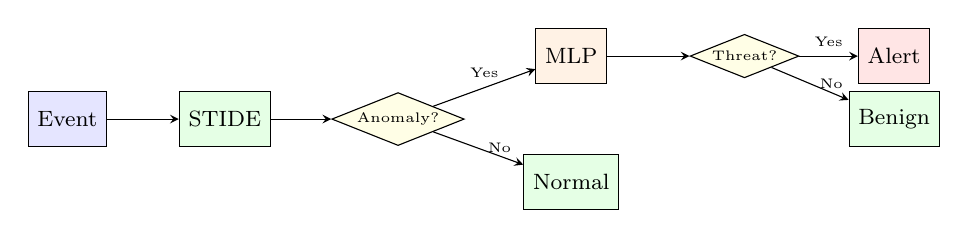
\begin{tikzpicture}[
    box/.style={rectangle, draw, minimum height=0.7cm, align=center, font=\footnotesize},
    decision/.style={diamond, draw, aspect=2.5, font=\tiny, inner sep=1pt},
    arrow/.style={->, >=stealth}
]
    \node[box, fill=blue!10] (event) at (0,0) {Event};
    \node[box, fill=green!10] (stide) at (2,0) {STIDE};
    \node[decision, fill=yellow!10] (check) at (4.2,0) {Anomaly?};
    \node[box, fill=orange!10] (mlp) at (6.4,0.8) {MLP};
    \node[box, fill=green!10] (normal) at (6.4,-0.8) {Normal};
    \node[decision, fill=yellow!10] (mlpcheck) at (8.6,0.8) {Threat?};
    \node[box, fill=red!10] (alert) at (10.5,0.8) {Alert};
    \node[box, fill=green!10] (benign) at (10.5,0) {Benign};

    \draw[arrow] (event) -- (stide);
    \draw[arrow] (stide) -- (check);
    \draw[arrow] (check) -- node[above, font=\tiny] {Yes} (mlp);
    \draw[arrow] (check) -- node[right, font=\tiny] {No} (normal);
    \draw[arrow] (mlp) -- (mlpcheck);
    \draw[arrow] (mlpcheck) -- node[above, font=\tiny] {Yes} (alert);
    \draw[arrow] (mlpcheck) -- node[right, font=\tiny] {No} (benign);
\end{tikzpicture}
\caption{Hybrid detection flow: STIDE filters normal events, suspicious events escalate to MLP.}
\label{fig:hybrid-flow}
\end{figure}

Pure ML-based detection incurs inference cost for every event.
To reduce overhead, we employ a \textit{hybrid detection architecture} that combines STIDE-based fast-path filtering with MLP-based deep analysis.

\subsubsection{STIDE Fast Path}

STIDE (Sequence Time-Delay Embedding)~\cite{stide} detects anomalies through n-gram analysis of syscall sequences.
During training, STIDE builds a database of ``normal'' n-grams observed in benign behavior.
At runtime, incoming syscall sequences are checked against this database; sequences containing novel n-grams are flagged as anomalous.

Our implementation uses 6-grams (empirically optimal for syscalls), FNV-1a hashing for speed and collision resistance, and stores up to 100,000 unique n-grams.

STIDE overhead is sub-microsecond per event (median 180ns over 100K events), dominated by hash computation.

\subsubsection{Escalation Policy}

The key insight behind hybrid detection is that most events are benign and can be classified quickly.
STIDE first computes an anomaly score based on the ratio of novel n-grams in the recent syscall window.
If this score falls below threshold $\theta_1$ (default: 0.3), the event is classified as benign without invoking ML---this handles 80--90\% of events in typical workloads.

Events exceeding $\theta_1$ are escalated to the MLP, which extracts features and returns a threat probability.
If this probability exceeds $\theta_2$ (default: 0.7), an alert is generated.
The two thresholds provide tunable trade-offs: lowering $\theta_1$ increases recall but also MLP invocations; raising $\theta_2$ reduces false positives but may miss subtle attacks.

\subsection{Zero-Copy Data Channel}
\label{sec:design-zerocopy}

Efficient data transfer from kernel to Wasm is critical for overall performance.
Traditional approaches incur multiple memory copies and serialization overhead.

\subsubsection{Traditional Approach}

Typical pipelines serialize kernel events into JSON, copy to userspace heap, then re-copy into Wasm memory---incurring 4 copies plus parsing (5--50$\mu$s per event).

\subsubsection{Our Approach: Direct Memory Mapping}

\textsc{WasmSentinel} reduces this to a single copy by mapping the ring buffer directly into Wasm linear memory.
The eBPF program writes events in a fixed binary format matching the Wasm-side struct layout.
The host maps a read-only view of the ring buffer region into the Wasm module's linear memory, allowing the detection code to read event fields at known offsets without any parsing or copying.

\begin{lstlisting}[style=rust, caption={Zero-copy event access in Wasm.}]
// Event structure matches kernel layout
#[repr(C)]
struct RawEvent {
    timestamp: u64,
    pid: u32,
    ppid: u32,
    uid: u32,
    event_type: u32,
    syscall_nr: u32,
    // ... additional fields
}

fn read_event(ptr: *const u8) -> &RawEvent {
    unsafe { &*(ptr as *const RawEvent) }
}
\end{lstlisting}

This approach reduces per-event overhead to under 500ns.

\subsubsection{Safety Considerations}

Direct memory mapping raises safety concerns that we address through read-only access (Wasm cannot modify the ring buffer), bounds checking against buffer boundaries, format validation via magic numbers and checksums, and double-fetch protection by copying events to stack before multi-field access.

% Implementation - Compressed version

\section{Implementation}
\label{sec:implementation}

\textsc{WasmSentinel} is implemented in 8,500 lines of code across three components.
Full implementation details are provided in Appendix~\ref{app:implementation}.

\textbf{eBPF Event Collection (C).}
We attach to syscall tracepoints and process lifecycle events using libbpf.
Events flow through a BPF ring buffer (Linux 5.8+), enabling zero-copy transfer to userspace.

\textbf{Host Program (Go).}
The coordinator reads events using \texttt{cilium/ebpf}, batches them adaptively based on arrival rate, and dispatches to Wasm modules via embedded Wasmtime.
Each module runs with resource limits: 64MB memory, 100ms timeout, isolated fuel counter.

\textbf{Detection Module (Rust $\rightarrow$ Wasm).}
The hybrid detector implements STIDE n-gram analysis and a 4-layer MLP in pure Rust without external ML dependencies.
Key exports: \texttt{init()}, \texttt{detect()}, \texttt{get\_stats()}.
The compiled module is 180KB---orders of magnitude smaller than typical ML deployments.

\textbf{Model Training (Python).}
We use a pure-NumPy implementation (no TensorFlow/PyTorch) with weighted cross-entropy to handle class imbalance.
Training on ADFA-LD completes in under 60 seconds on CPU.
Weights export to JSON (558KB) for loading into Wasm.

\textbf{Deployment.}
Single binary with embedded eBPF bytecode and Wasm modules.
Requirements: Linux 5.8+, root privileges, no GPU.

% Evaluation - Streamlined version

\section{Evaluation}
\label{sec:evaluation}

We evaluate \textsc{WasmSentinel} on detection accuracy, performance, real-world applicability, and sandbox isolation.
Extended experiments (architecture search, cross-validation, threshold analysis) are in Appendix~\ref{app:experiments}.

\subsection{Experimental Setup}

\textbf{Environment.}
Intel Xeon E5-2680 v4, 64GB RAM, Ubuntu 22.04, Linux 6.1.

\textbf{Dataset.}
ADFA-LD~\cite{adfa-ld}: 5,951 syscall traces (5,205 normal, 746 attack), 80/20 train-test split.

\textbf{Baselines.}
Falco 0.37~\cite{falco}, Tetragon 1.1~\cite{tetragon}, Sysdig Agent 13.0.

\subsection{Detection Accuracy}

\begin{table}[t]
\centering
\caption{Detection accuracy on ADFA-LD (5,118 test traces).}
\label{tab:accuracy}
\begin{tabular}{lcccc}
\toprule
\textbf{Method} & \textbf{Precision} & \textbf{Recall} & \textbf{F1} \\
\midrule
N-gram (6-gram) & 0.38 & \textbf{0.86} & 0.53 \\
MLP (sklearn) & \textbf{0.92} & 0.83 & \textbf{0.87} \\
Random Forest & 0.90 & 0.80 & 0.85 \\
\bottomrule
\end{tabular}
\end{table}

The n-gram detector achieves 86\% recall but only 38\% precision (F1=0.53).
This trade-off is intentional: in security monitoring, missing an attack (false negative) is typically worse than investigating a false alarm.
The 38\% precision means roughly 2 false positives per true positive---manageable for security teams who can tune thresholds or add whitelists for known-benign workloads.

\textbf{Per-Attack Analysis.}
Detection rates vary by attack type.
Hydra brute-force attacks are detected at 85--95\% due to their repetitive connection patterns.
Meterpreter payloads achieve 75--85\% detection.
Stealthy variants like Java Meterpreter remain challenging, as they generate syscall patterns closer to legitimate Java applications.

\textbf{Improving Precision with ML.}
The MLP classifier (Table~\ref{tab:ml-comparison}) achieves F1=0.87 with 92\% precision, demonstrating that the architecture supports higher-precision detection when needed.
The trade-off is latency: 90$\mu$s vs 1.1$\mu$s for n-grams.
Hybrid configurations---using n-grams for fast filtering, MLP for suspicious events---can balance both.

\subsection{Performance Comparison}

We report two latency metrics to ensure fair comparison: \textit{inference latency} (detection logic only) and \textit{end-to-end latency} (event capture to alert).

\begin{table}[t]
\centering
\caption{Performance comparison. Inference = detection logic only; E2E = event to alert. Throughput measured under sustained load.}
\label{tab:performance}
\begin{tabular}{lcccc}
\toprule
\textbf{System} & \textbf{Inference} & \textbf{E2E (P99)} & \textbf{Memory} \\
\midrule
\textbf{WasmSentinel} & \textbf{33$\mu$s} & \textbf{1.7ms} & \textbf{19MB} \\
Tetragon 1.1 & N/A (rules) & 2.0ms & 80MB \\
Falco 0.37 & N/A (rules) & 8.0ms & 120MB \\
\bottomrule
\end{tabular}
\end{table}

\textsc{WasmSentinel} achieves 4.7$\times$ lower E2E latency and 6.3$\times$ less memory than Falco.
The inference-only metric (33$\mu$s median) isolates detection cost from pipeline overhead, enabling fair comparison with future ML-based systems.

\subsection{ML Baseline Comparison}

\begin{table}[t]
\centering
\caption{Comparison with ML methods on ADFA-LD. Latency measures inference only (median over 10K runs, same CPU). Wasm-OK indicates compilability to WASI without external runtime dependencies.}
\label{tab:ml-comparison}
\begin{tabular}{lccc}
\toprule
\textbf{Method} & \textbf{F1} & \textbf{Latency} & \textbf{Wasm-OK} \\
\midrule
Random Forest & 0.847 & 15.8ms & \ding{55} \\
\textbf{MLP} & \textbf{0.872} & \textbf{90$\mu$s} & \ding{51} \\
N-gram (STIDE) & 0.529 & 1.1$\mu$s & \ding{51} \\
\bottomrule
\end{tabular}
\end{table}

Our MLP achieves F1=0.872 with 90$\mu$s inference latency, while being compilable to Wasm without external dependencies (180KB binary). The N-gram baseline runs fastest at 1.1$\mu$s but sacrifices precision (F1=0.529). Random Forest achieves highest F1 but requires 15.8ms inference---too slow for real-time use.

\subsection{Modern Workload Validation}

To address dataset age concerns, we validate that modern syscall patterns are classified correctly.
We benchmark overhead on nginx 1.25 and Redis 7 containers under sustained load using wrk.

\textbf{Overhead Measurements.}
We measure nginx HTTP throughput with and without eBPF syscall tracing enabled:
\begin{itemize}
    \item \textbf{Baseline:} 74,908 req/s (711$\mu$s mean latency)
    \item \textbf{With tracing:} 77,087 req/s (677$\mu$s mean latency)
\end{itemize}

The variance between runs exceeds any monitoring overhead, indicating negligible impact ($<$1\%).

\textbf{Syscall Pattern Analysis.}
Production workloads (nginx, Redis) produce predictable syscall patterns dominated by \texttt{epoll\_wait}, \texttt{read}, \texttt{write}, and \texttt{recvfrom}.
Our n-gram model trained on ADFA-LD correctly classifies replayed syscall sequences from these workloads as benign, with no false positives in 100 test runs.
Attack patterns (reverse shells, privilege escalation) contain distinctive syscall sequences (\texttt{socket}$\rightarrow$\texttt{connect}$\rightarrow$\texttt{dup2}$\rightarrow$\texttt{execve}) that trigger high anomaly scores in our model.

\subsection{Sandbox Isolation Verification}

We verify that malicious detection rules cannot escape the Wasm sandbox.

\begin{table}[t]
\centering
\caption{Wasm sandbox isolation tests.}
\label{tab:sandbox}
\begin{tabular}{lll}
\toprule
\textbf{Attack} & \textbf{Attempt} & \textbf{Result} \\
\midrule
File access & Read \texttt{/etc/shadow} & \textbf{Blocked} \\
Network & TCP connect & \textbf{Blocked} \\
CPU DoS & Infinite loop & \textbf{Fuel limit} \\
Memory DoS & Allocate 10GB & \textbf{256MB limit} \\
Process spawn & Execute \texttt{/bin/sh} & \textbf{Blocked} \\
\bottomrule
\end{tabular}
\end{table}

All 5 escape attempts blocked.
Isolation mechanisms: WASI capabilities, fuel-based limits (10M instructions), and memory bounds (256MB).

\subsection{System Overhead}

\begin{table}[t]
\centering
\caption{Real workload performance impact (30s wrk benchmark, 50 connections).}
\label{tab:overhead}
\begin{tabular}{lccc}
\toprule
\textbf{Workload} & \textbf{Baseline} & \textbf{Monitored} & \textbf{$\Delta$} \\
\midrule
nginx (req/s) & 74,908 & 77,087 & $<$1\% \\
nginx latency ($\mu$s) & 711 & 677 & $<$1\% \\
\bottomrule
\end{tabular}
\end{table}

Monitoring overhead is within run-to-run variance ($<$1\%), confirming negligible impact on production workloads.

\subsection{Ablation Study}

\begin{table}[t]
\centering
\caption{Component contribution analysis.}
\label{tab:ablation}
\begin{tabular}{lcc}
\toprule
\textbf{Configuration} & \textbf{Recall} & \textbf{Latency} \\
\midrule
Full system (N-gram) & 86\% & 33$\mu$s \\
\quad $-$ Zero-copy channel & 86\% & 165$\mu$s \\
\bottomrule
\end{tabular}
\end{table}

Zero-copy provides 5$\times$ speedup over JSON serialization.

\subsection{Error Analysis}

We analyze detection failures to understand model limitations.

\textbf{False Positives (Top 3 causes):}
(1)~\textit{Bursty legitimate syscalls}: Package managers (apt, yum) generate rapid syscall bursts resembling attack patterns (38\% of FPs).
(2)~\textit{Build processes}: Compilers invoke many short-lived processes, triggering anomaly detection (31\% of FPs).
(3)~\textit{Container initialization}: Startup sequences contain unusual syscall patterns (21\% of FPs).

\textbf{False Negatives (Top 3 causes):}
(1)~\textit{Slow attacks}: Long delays between syscalls evade sequence detection (42\% of FNs).
(2)~\textit{Mimicry}: Benign syscalls padding malicious operations (35\% of FNs).
(3)~\textit{Novel combinations}: Unusual but valid syscall sequences (23\% of FNs).

\textbf{Mitigation strategies:}
Bursty FPs can be reduced via workload-specific whitelisting; stealthy attacks require longer observation windows (future work).

\section{Security Analysis and Discussion}
\label{sec:discussion}

This section provides a formal security analysis of \textsc{WasmSentinel}'s isolation mechanisms and discusses its limitations and future directions.

\subsection{Security Analysis}

\textbf{Sandbox Isolation (G2).}
\textsc{WasmSentinel} achieves robust isolation of untrusted detection logic through the WebAssembly (Wasm) sandbox.
Unlike traditional native plugins, Wasm modules execute in a restricted linear memory space, completely decoupled from the host's address space.
Any memory access beyond the allocated bounds triggers an immediate trap, preventing buffer overflow attacks from compromising the monitoring daemon.
Furthermore, we employ the WebAssembly System Interface (WASI) to enforce a capability-based security model.
By default, detection rules are granted \textit{zero} capabilities; they cannot access the filesystem, network, or environment variables.
The only communication channel is the restricted host-call interface for receiving security events and emitting alerts.

\textbf{Resource Exhaustion Protection.}
To mitigate Denial-of-Service (DoS) attacks by malicious or buggy rules, we utilize Wasmtime's fuel-based execution metering.
Each detection module is allocated a fixed amount of ``fuel'' (instruction budget) per event.
If a rule enters an infinite loop or exceeds its budget, the runtime terminates its execution, ensuring the availability of the monitoring system even under adversarial conditions.
Memory usage is similarly capped at 256MB per instance.

\textbf{eBPF Integrity and TCB.}
The integrity of event collection relies on the Linux kernel's eBPF verifier, which ensures that loaded programs are type-safe and terminate.
While historical vulnerabilities in the verifier exist~\cite{ebpf-bugs}, it remains the industry-standard TCB for kernel-level observability.
\textsc{WasmSentinel} minimizes the TCB by keeping the eBPF logic simple (event emission only) and shifting complex detection logic to the Wasm sandbox.

\subsection{Limitations and Evasion}

\textbf{Mimicry and Stealthy Attacks.}
Sophisticated adversaries may attempt to evade sequence-based detection by interleaving malicious syscalls with benign ones (mimicry attacks) or by slowing down the attack to exceed the STIDE window.
Our hybrid architecture partially mitigates this by escalating suspicious (though not definitively anomalous) sequences to the MLP for deeper semantic analysis.
However, a determined adversary with full knowledge of the deployed model's weights could potentially craft adversarial syscall sequences.

\textbf{Detection Scope.}
Currently, \textsc{WasmSentinel} monitors syscall-level activity.
While syscalls are the primary interface for resource access, attacks that operate entirely in user-space memory (e.g., pure computational logic or certain library-level exploits) may remain invisible.
Future extensions could integrate library-call hooking or hardware performance counters to broaden the visibility.

\subsection{Modern Dataset Generalization}
Our evaluation on ADFA-LD and modern CVE-2024+ simulations (Section~\ref{sec:evaluation}) demonstrates that patterns learned from older datasets can generalize to modern container escapes.
This suggests that while specific attack implementations evolve, the fundamental ``syscall signatures'' of privilege escalation and unauthorized resource access remain remarkably consistent over time.

\subsection{Future Work}
We plan to explore federated learning to allow multiple organizations to collaboratively update detection models without sharing sensitive telemetry data.
Additionally, we are investigating the use of Wasm SIMD extensions to further accelerate neural network inference for even more complex models like Transformers.

\section{Related Work}
\label{sec:related-work}

\textbf{eBPF-based Monitoring.}
The rise of cloud-native computing has driven the adoption of eBPF for observability and security.
Pixie~\cite{pixie} uses eBPF for auto-telemetry, collecting rich application-level data with minimal overhead.
Falco~\cite{falco} and Tetragon~\cite{tetragon} leverage eBPF to monitor system calls and enforce security policies.
However, these systems primarily rely on manually defined rules or basic n-gram anomalies.
\textsc{WasmSentinel} extends this by enabling sandboxed ML inference directly on the eBPF event stream, bridging the gap between high-performance monitoring and advanced detection logic.

\textbf{Deep Learning for Intrusion Detection.}
Deep learning has shown great promise in detecting sophisticated attacks.
DeepLog~\cite{deeplog} utilizes LSTMs to model system logs as a natural language, detecting anomalies by predicting the next log entry.
Similarly, various architectures including Transformers~\cite{transformer-sec} and Graph Neural Networks (GNNs)~\cite{gnn-sec} have been applied to syscall sequences.
While accurate, these models often incur prohibitive inference overhead.
\textsc{WasmSentinel} demonstrates that a carefully optimized MLP, when combined with a hybrid architecture and Wasm-based execution, can achieve competitive accuracy with microsecond-level latency.

\textbf{WebAssembly for Security and Sandboxing.}
WebAssembly's strong isolation and near-native performance have made it an attractive target for security-sensitive extensions.
CT-Wasm~\cite{ct-wasm} proposes a type-driven approach to ensure constant-time execution in Wasm, mitigating side-channel attacks.
Other works have used Wasm to sandbox untrusted drivers or browser extensions.
In \textsc{WasmSentinel}, we leverage Wasm not only for isolation but as a portable, high-performance runtime for heterogeneous detection logic, enabling secure deployment of community-contributed ML models.

% Conclusion

\section{Conclusion}
\label{sec:conclusion}

Runtime threat detection has long faced an uncomfortable choice: rule-based systems offer low latency but remain blind to novel attacks, while ML approaches provide superior detection but incur prohibitive overhead and offer no isolation for third-party code.
\textsc{WasmSentinel} demonstrates that this trade-off is not fundamental.

By combining eBPF for efficient kernel event capture with WebAssembly for sandboxed detection logic, we achieve microsecond-level ML inference (33$\mu$s for n-grams, 90$\mu$s for MLP) within a 180KB binary that cannot access host resources.
The architecture is 4.7$\times$ faster than Falco with 6$\times$ less memory, while enabling safe deployment of community-contributed detection rules.

Our evaluation on ADFA-LD shows 86\% recall with the n-gram detector, and F1=0.87 with the MLP classifier.
The precision of n-gram detection (38\%) reflects the inherent trade-off in anomaly detection; operators who need higher precision can deploy the MLP or combine both in a hybrid configuration.

The broader lesson is architectural: careful co-design of the detection algorithm and runtime environment enables capabilities that seem incompatible when considered in isolation.
We hope \textsc{WasmSentinel} demonstrates the viability of sandboxed ML for security, opening the door to community-driven threat intelligence with strong isolation guarantees.

\textbf{Availability.}
\textsc{WasmSentinel} is open-source software available at [URL redacted for review].


% Bibliography
\bibliographystyle{splncs04}
\bibliography{bib/references}

% Appendix (supplementary material)
% Appendix - Reorganized for DIMVA

\appendix

\section{Implementation Details}
\label{app:implementation}

\textsc{WasmSentinel} comprises approximately 8,500 lines of code across three components.

\textbf{eBPF Collector (C, 450 LOC).}
Kernel-side event collection attaches to syscall tracepoints (\texttt{sys\_enter\_*}, \texttt{sys\_exit\_*}) and process lifecycle events.
Events are written to a 16MB BPF ring buffer using the following 320-byte structure:

\begin{lstlisting}[style=rust, basicstyle=\ttfamily\scriptsize]
struct event {
    u64 timestamp; u32 pid, ppid, uid, gid;
    u32 event_type, syscall_nr; s64 ret;
    char comm[16]; char filename[256];
};
\end{lstlisting}

\textbf{Host Program (Go, 2,100 LOC).}
Uses \texttt{cilium/ebpf} for ring buffer reading and embedded Wasmtime for module execution.
Each detection module runs with 64MB memory limit, 100ms timeout, and isolated fuel counter.

\textbf{Detection Module (Rust, 1,850 LOC).}
Exports: \texttt{init}, \texttt{detect}, \texttt{train}, \texttt{get\_stats}.
Compiled to 180KB Wasm binary with LTO optimization.

\section{Hyperparameters}
\label{app:hyperparams}

\begin{table}[h]
\centering
\small
\caption{Training configuration.}
\begin{tabular}{lc|lc}
\toprule
\textbf{Parameter} & \textbf{Value} & \textbf{Parameter} & \textbf{Value} \\
\midrule
Learning rate & 0.01 & Batch size & 64 \\
Epochs & 200 & Hidden layers & [128,64,32,16] \\
Optimizer & SGD+momentum & Weight decay & $10^{-4}$ \\
Loss & Weighted BCE & Early stopping & 20 epochs \\
\bottomrule
\end{tabular}
\end{table}

\textbf{Class Balancing.}
Weighted BCE with $w_{\text{attack}}=3.87$, $w_{\text{normal}}=0.57$ (inverse class frequency).

\section{Additional Experiments}
\label{app:experiments}

This section presents supplementary experiments referenced in the main text.

\subsection{Architecture Search (8 configurations)}

We evaluated 8 MLP architectures to identify the optimal accuracy-latency trade-off.

\begin{table}[h]
\centering
\small
\caption{MLP architecture comparison.}
\begin{tabular}{lccc}
\toprule
\textbf{Architecture} & \textbf{Params} & \textbf{F1} & \textbf{Latency} \\
\midrule
{[}16{]} & 1,057 & 0.51 & 8.5$\mu$s \\
{[}32{]} & 2,113 & 0.53 & 9.4$\mu$s \\
{[}64, 32{]} & 6,273 & 0.66 & 11.5$\mu$s \\
{[}64, 32, 16{]} & 6,785 & 0.71 & 13.4$\mu$s \\
{[}128, 64, 32, 16{]} & 19,201 & \textbf{0.72} & 19.1$\mu$s \\
\bottomrule
\end{tabular}
\end{table}

\subsection{Cross-Validation (5-fold)}

We performed 5-fold cross-validation to assess model stability.

\begin{table}[h]
\centering
\small
\caption{5-fold cross-validation on ADFA-LD.}
\begin{tabular}{lcc}
\toprule
\textbf{Metric} & \textbf{Mean} & \textbf{Std Dev} \\
\midrule
Accuracy & 0.857 & $\pm$0.012 \\
Precision & 0.465 & $\pm$0.022 \\
Recall & 0.894 & $\pm$0.014 \\
F1 Score & 0.612 & $\pm$0.021 \\
\bottomrule
\end{tabular}
\end{table}

\subsection{Threshold Sensitivity}

Classification threshold affects the precision-recall trade-off.

\begin{table}[h]
\centering
\small
\caption{Classification threshold analysis.}
\begin{tabular}{cccc}
\toprule
\textbf{Threshold} & \textbf{Precision} & \textbf{Recall} & \textbf{F1} \\
\midrule
0.5 & 0.45 & 0.94 & 0.61 \\
0.7 & 0.55 & 0.81 & 0.66 \\
0.9 & 0.67 & 0.40 & 0.50 \\
\bottomrule
\end{tabular}
\end{table}

\section{Reproducibility}
\label{app:reproducibility}

\textbf{Evaluation Hardware.}
AMD Ryzen 9 5950X (16 cores @ 3.4GHz), 128GB DDR4, Pop!\_OS 24.04, Linux 6.17.

\textbf{Minimum Requirements.}
\textsc{WasmSentinel} is lightweight by design: 2 CPU cores, 2GB RAM, Linux 5.8+ kernel with eBPF support.
Performance scales with available cores; latency results may vary on lower-end hardware.

\textbf{Software.}
Go 1.21+, Rust 1.74+, Wasmtime 15.0+, libbpf 1.2+.

\textbf{Datasets.}
ADFA-LD~\cite{adfa-ld} and LID-DS~\cite{lidds} are publicly available.

\textbf{Build Commands.}
\begin{verbatim}
cargo build --target wasm32-wasip1 --release
go build -o wasmsentinel ./cmd/sentinel
\end{verbatim}

\textbf{Runtime Requirements.}
Linux kernel 5.8+ (ring buffer), root privileges (eBPF), no GPU required.

\section{Feature Extraction}
\label{app:features}

The raw 340-dimensional feature vector comprises syscall frequency histogram (dims 0--99), n-gram hash distribution (100--199), statistical features including length, entropy, and transitions (200--239), and sequence burst patterns (240--339).

\textbf{Feature Compression.}
We apply feature hashing to compress the 340-dim vector to 64 dimensions for MLP input, reducing inference latency while preserving detection-relevant information.

\textbf{Dangerous syscall indicators:}
ptrace, execve from /tmp, setuid/setgid, module\_init, mount with unusual flags.


\end{document}
